\documentclass[12pt]{article}
\usepackage[margin=1in]{geometry}
\usepackage{subcaption}
\usepackage{graphicx}
\usepackage{placeins}
\usepackage{amsmath}
\usepackage{url}
\usepackage{cite}


% acronyms for text or math mode
% \newcommand {\ccast} {\mbox{\small\textsc{ccast}}}
\newcommand {\ccast} {\mbox{\small CCAST}}
\newcommand {\nedn} {\mbox{\small NEdN}}
\newcommand {\kcarta} {\mbox{k\small{CARTA}}}

\newcommand {\chirp} {\mbox{\small CHIRP}}
\newcommand {\cris}  {\mbox{\small CrIS}}
\newcommand {\airs}  {\mbox{\small AIRS}}
\newcommand {\iasi}  {\mbox{\small IASI}}
\newcommand {\idps}  {\mbox{\small IDPS}}
\newcommand {\nasa}  {\mbox{\small NASA}}
\newcommand {\noaa}  {\mbox{\small NOAA}}
\newcommand {\nstar} {\mbox{\small STAR}}
\newcommand {\umbc}  {\mbox{\small UMBC}}
\newcommand {\uw}    {\mbox{\small UW}}

\newcommand {\fft}  {\mbox{\small FFT}}
\newcommand {\ifft} {\mbox{\small IFFT}}
\newcommand {\fir}  {\mbox{\small FIR}}
\newcommand {\fov}  {\mbox{\small FOV}}
\newcommand {\for}  {\mbox{\small FOR}}
\newcommand {\ict}  {\mbox{\small ICT}}
\newcommand {\ils}  {\mbox{\small ILS}}
\newcommand {\igm}  {\mbox{\small IGM}}
\newcommand {\opd}  {\mbox{\small OPD}}
\newcommand {\rms}  {\mbox{\small RMS}}
\newcommand {\zpd}  {\mbox{\small ZPD}}
\newcommand {\ppm}  {\mbox{\small PPM}}
\newcommand {\srf}  {\mbox{\small SRF}}
\newcommand {\sdr}  {\mbox{\small SDR}}
\newcommand {\FWHM} {\mbox{\small FWHM}}
\newcommand {\fwhm} {\mbox{\small\textsc{fwhm}}}

\newcommand {\ES} {\mbox{\small ES}}
\newcommand {\SP} {\mbox{\small SP}}
\newcommand {\IT} {\mbox{\small IT}}
\newcommand {\SA} {\mbox{\small SA}}

\newcommand {\ET} {\mbox{\small ET}}
\newcommand {\FT} {\mbox{\small FT}}

\newcommand {\wn} {\mbox{cm$^{-1}$}}
\newcommand {\cm} {\mbox{cm}}

% abbreviations, mainly for math mode
\newcommand {\real} {\mbox{real}}
\newcommand {\imag} {\mbox{imag}}
\newcommand {\atan} {\mbox{atan}}
\newcommand {\obs}  {\mbox{obs}}
\newcommand {\calc} {\mbox{calc}}
\newcommand {\sinc} {\mbox{sinc}}
\newcommand {\psinc} {\mbox{psinc}}
\newcommand {\std} {\mbox{std}}
\newcommand {\nchan} {\mbox{nchan}}
\newcommand {\nobs} {\mbox{nobs}}

% symbols, for math mode only
\newcommand {\lmax} {L_{\mbox{\tiny max}}}
\newcommand {\vmax} {V_{\mbox{\tiny max}}}

\newcommand {\tauobs} {\tau_{\mbox{\tiny obs}}}
\newcommand {\taucal} {\tau_{\mbox{\tiny calc}}}
\newcommand {\Vdc}  {V_{\mbox{\tiny DC}}}

\newcommand {\rIT} {r_{\mbox{\tiny\textsc{ict}}}}
\newcommand {\rES} {r_{\mbox{\tiny\textsc{es}}}}
\newcommand {\robs} {r_{\mbox{\tiny obs}}}

\newcommand {\rITobs} {r_{\mbox{\tiny\textsc{ict}}}^{\mbox{\tiny obs}}}
\newcommand {\rITcal} {r_{\mbox{\tiny\textsc{ict}}}^{\mbox{\tiny cal}}}

\newcommand {\rESuser} {r_{\mbox{\tiny\textsc{es}}}^{\mbox{\tiny user}}}
\newcommand {\rITuser} {r_{\mbox{\tiny\textsc{ict}}}^{\mbox{\tiny user}}}
\newcommand {\rITsensor} {r_{\mbox{\tiny\textsc{ict}}}^{\mbox{\tiny sensor}}}
\newcommand {\rITfov} {r_{\mbox{\tiny\textsc{ict}}}^{\mbox{\tiny fov}}}

\newcommand {\fcos} {f_{\mbox{\tiny cos}}}
\newcommand {\fatbd} {f_{\mbox{\tiny\textsc{atbd}}}}

\newcommand {\ITmean} {\langle\mbox{\small IT}\rangle}
\newcommand {\SPmean} {\langle\mbox{\small SP}\rangle}

\newcommand {\Ttc} {t^{\mbox{\tiny\textsc{tc}}}}
\newcommand {\Tac} {t^{\mbox{\tiny\textsc{ac}}}}
\newcommand {\rtc} {r_{\mbox{\tiny\textsc{tc}}}}
\newcommand {\rta} {r_{\mbox{\tiny\textsc{ta}}}}



\title{
  CHIRP Users Guide \\
}
\author{H.~E.~Motteler and L.~L.~Strow \\
  \\
  UMBC Atmospheric Spectroscopy Lab \\
  Joint Center for Earth Systems Technology \\
}
\date{\today}
\begin{document}
\maketitle

% introduction and overview
% radiances
% file format and data organization
% QC and NEdN

%----------- section --------------------------------------------------%
\section{Introduction}

Spectra of the earth's thermal emission as measured by the AIRS,
CrIS, and IASI hyper-spectral sounders are becoming a significant
part of the long term climate record.  These instruments have
broadly similar spatial sampling, spectral resolution, and band
spans.  However the spectral response functions differ in detail,
leading to significant differences in observed spectra.

The CHIRP product provides a single, combined record of this data,
by taking advantage of the similar spatial sampling and translating
AIRS and CrIS radiances to a common format.  The translation from
CrIS to CHIRP is straightforward.  The translation from AIRS to CrIS
has some novel features.  AIRS is a grating spectrometer with a
distinct response function for each channel, whereas CrIS is a
Michaelson interferometer with a sinc response function.  We use our
detailed knowledge of the AIRS spectral response functions to
deconvolve AIRS channel radiances to a resolution enhanced
intermediate representation that is then reconvolved to the CHIRP
specifications.

The CHIRP record starts with AIRS data from Fall 2002, and will
cross over to CrIS SNPP or NOAA-20 and continue in the future with
NOAA-21, 22, etc., with sounder crossover dates to be determined.
These sounders share a PM equatorial crossing time and will become
the CHIRP-1330 product.  Although the primary product is a single
record, support products in the form of translations for other NOAA
sounders may also be provided.  CHIRP-1330 is made available by JPL
Sounder SIPS as a product at the GSFC-DIS.  In the future, we plan
to add IASI, for a CHIRP-1030 product.

The Users Guide has three main sections, the CHIRP radiance
specifications, CHIRP file format and data organization, and CHIRP
QC and NEdN.  The most commonly used fields are discussed in the
file format section, with detailed descriptions of all field and
attribute specs summarized in an appendix.

%----------- section --------------------------------------------------%
\section{CHIRP Radiances}

CHIRP radiances are for a nominal 3-band interferometer with an
{\opd} of $0.8$ {\cm} in the long-wave (LW), $0.6$ {\cm} in the
medium-wave (MW), and $0.4$ {\cm} in the short-wave (SW) band, with
a Hamming apodization applied as part of the product spec.  The MW
and SW resolutions are lower than the CrIS-parent OPD of $0.8$ {\cm}
for all three bands, and were chosen to to give an approximate match
to the AIR resolution in the MW and SW.

After translation from CrIS the three bands have 713, 649, and 317
channels, respectively.  These are concatenated for the CHIRP
product, for a total of 1679 channels withfrequency steps of $1/(2
\hbox{ OPD})$.  The \texttt{wnum} field is a 1679-vector which gives
channel frequencies, and \texttt{rad} is a 1679 by 12150 array of
radiance data.  (The dimension 12150 is the number of observations
in a granule, and is defined in the next section.)

AIRS-parent CHIRP uses the same channel set.  However the
AIRS-to-CHIRP translation gives only 1483 channels, due to slightly
different band spans.  These are embedded in the 1679 channel set,
with missing channels flagged, as described in section \ref{secQC}.

Figure \ref{figA} shows AIRS and AIRS-parent CHIRP spectra, granule
means for 19 Aug 2018 granule 25.  The CHIRP bands are the
intersection of the AIRS and CrIS bands.  Figure \ref{figB} is a MW
detail from Figure \ref{figA}.  Note that the data are on two
different grids, and what we mainly see is the effect of the CHIRP
apodization.

The CHIRP ILS is the Hamming-apodized sinc ILS for $0.8$ {\cm} (LW),
$0.6$ {\cm} (MW), and $0.4$ {\cm} (SW) {\opd}s, and is the same for
the AIRS and CrIS parent data.  Figure \ref{figC} shows a typical MW
CHIRP ILS.  For AIRS-parent CHIRP, we show the AIRS channel weights
for this CHIRP channel, paired with the corresponding AIRS SRFs,
normalized to the weight values.

% The weights are from a row of a linearized approximation of the
% AIRS to CrIS translation.

% % sample AIRS and CHIRP spectra
% \begin{figure} 
% \centering
% 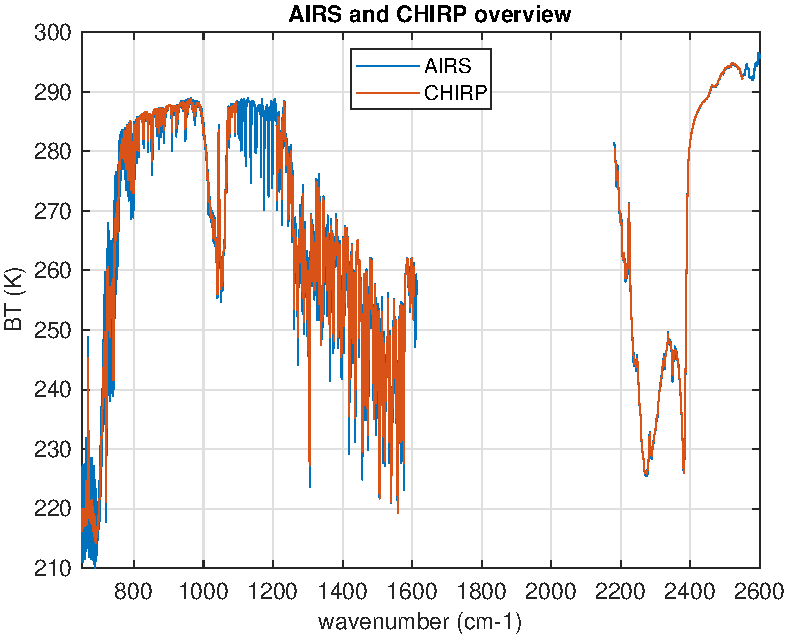
\includegraphics[height=7cm]{figures/airs_and_chirp_overview.pdf}
% \caption{Sample AIRS and AIRS-parent CHIRP spectra, granule means
%   for 19 Aug 2018 granule 25.  The CHIRP bands are the intersection
%   of the AIRS and CrIS bands.}
% \label{figA}
% \end{figure}
% 
% % sample AIRS and CHIRP spectra (detail)
% \begin{figure} 
% \centering
% 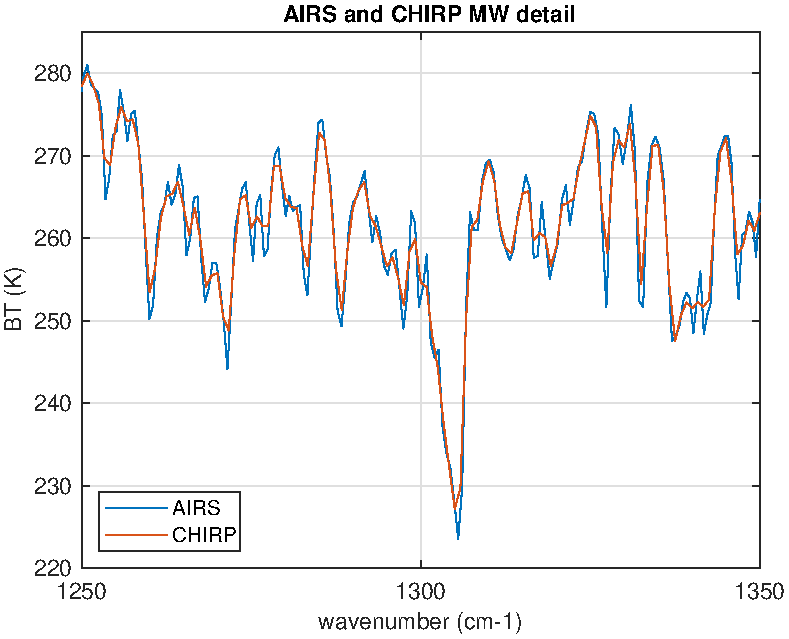
\includegraphics[height=7cm]{figures/airs_and_chirp_mw_detail.pdf}
% \caption{MW detail from the same granule.  Note that the data are on
%   two different grids, and what we mainly see is the effect of the
%   CHIRP apodization.}
% \label{figB}
% \end{figure}

\begin{figure}
  \begin{subfigure}[b]{0.45\textwidth}
    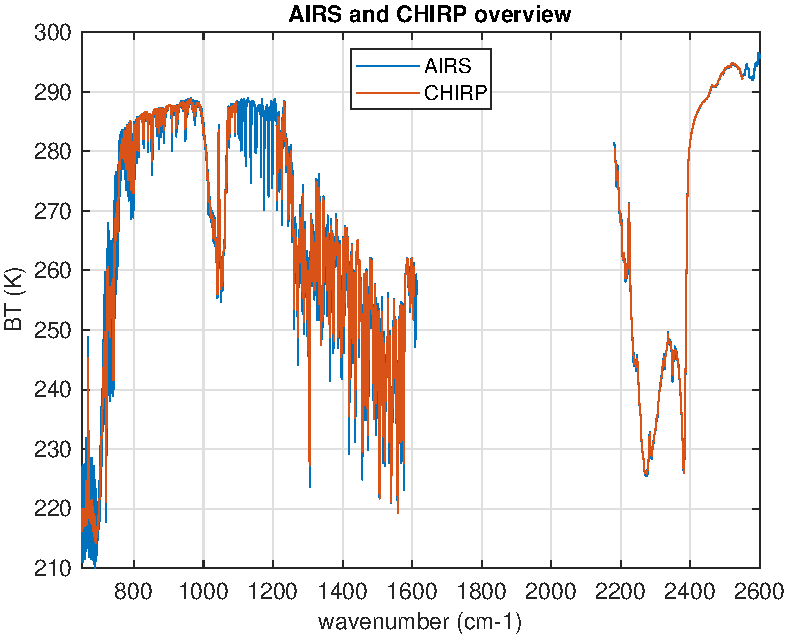
\includegraphics[width=\textwidth]{figures/airs_and_chirp_overview.pdf}
    \caption{Sample AIRS and AIRS-parent CHIRP spectra, granule means
      for 19 Aug 2018 granule 25.  The CHIRP bands are the intersection
      of the AIRS and CrIS bands.}
    \label{figA}
  \end{subfigure}
  \hskip5mm
  \begin{subfigure}[b]{0.45\textwidth}
    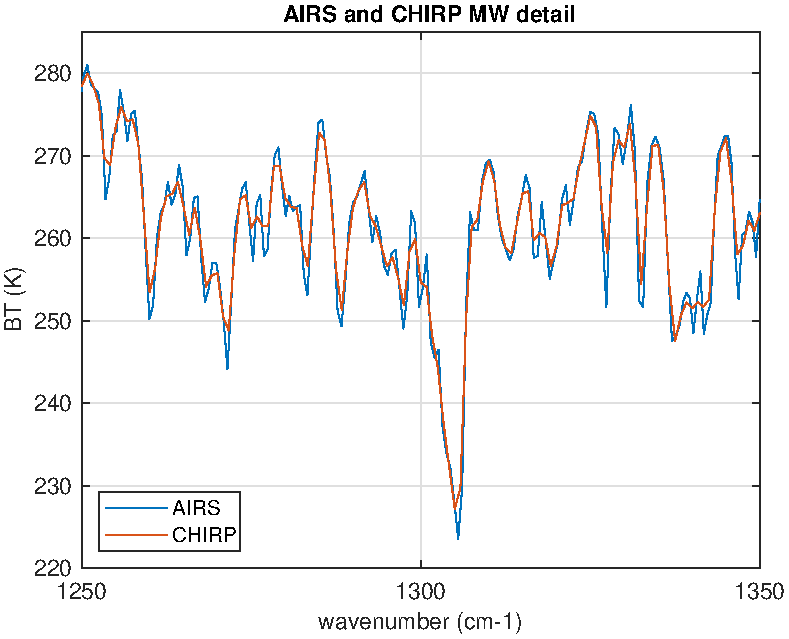
\includegraphics[width=\textwidth]{figures/airs_and_chirp_mw_detail.pdf}
    \caption{MW detail from the same granule.  Note that the data
      are on two different grids, and what we mainly see is the
      effect of the CHIRP apodization.}
    \label{figB}
  \end{subfigure}
\end{figure}

% CHIRP sample ILS
\begin{figure} % source a2cris_srfs.m
\centering
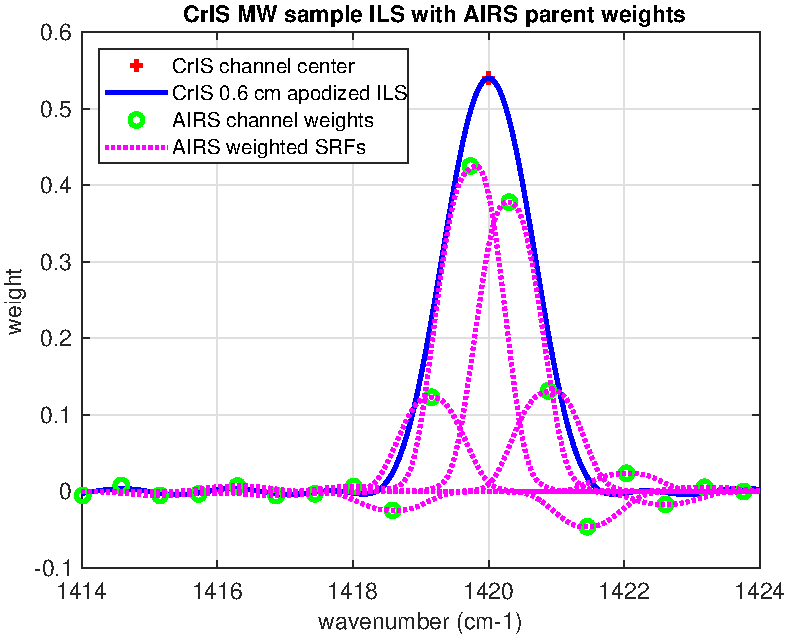
\includegraphics[width=\textwidth]{figures/sample_CrIS_ILS_with_AIRS_parent_SRFs.pdf}
\caption{The MW CHIRP apodized ILS, together with weights for the
  AIRS channels, for the CHIRP channel shown.  The AIRS weights are
  paired with the corresponding AIRS SRFs, normalized to the weight
  values.}
\label{figC}
\end{figure}

\subsection{The Translations}

\begin{itemize}

  \item For the AIRS to CHIRP translation, we deconvolve
    AIRS to an intermediate grid, typically $0.1$ {\wn}, with a
    Moore-Penrose pseudo-inverse of tabulated AIRS SRFs, and then
    reconvolve to the CrIS ``mid res'' (aka \chirp) user grid via
    resampling or double Fourier interpolation.

  \item This is described in detail in ``AIRS deconvolution and
    the translation of AIRS-to-CrIS radiances with applications
    for the IR climate record,'' IEEE Transactions on Geoscience and
    Remote Sensing, 57(3):1793--1803, 2018.

  \item The CrIS to CHIRP translation is done by interpolation
    from the CrIS high res product (0.8/0.8/0.8 cm \opd).  CHIRP
    can also be produced directly by {\umbc} {\ccast} (CrIS L0 to
    L1b processing), with a single interpolation from the sensor to
    the CHIRP user grid.

  \item Hamming apodization and an optional bias correction are
    applied to both translations.  Currently AIRS and CrIS J1
    parent are adjusted to match CrIS SNPP.

\end{itemize}

%----------- section --------------------------------------------------%
\section{CHIRP Data Format}

% one day track map
\begin{figure} % source plot_subpt.m
% \hskip-3.5cm
\centering
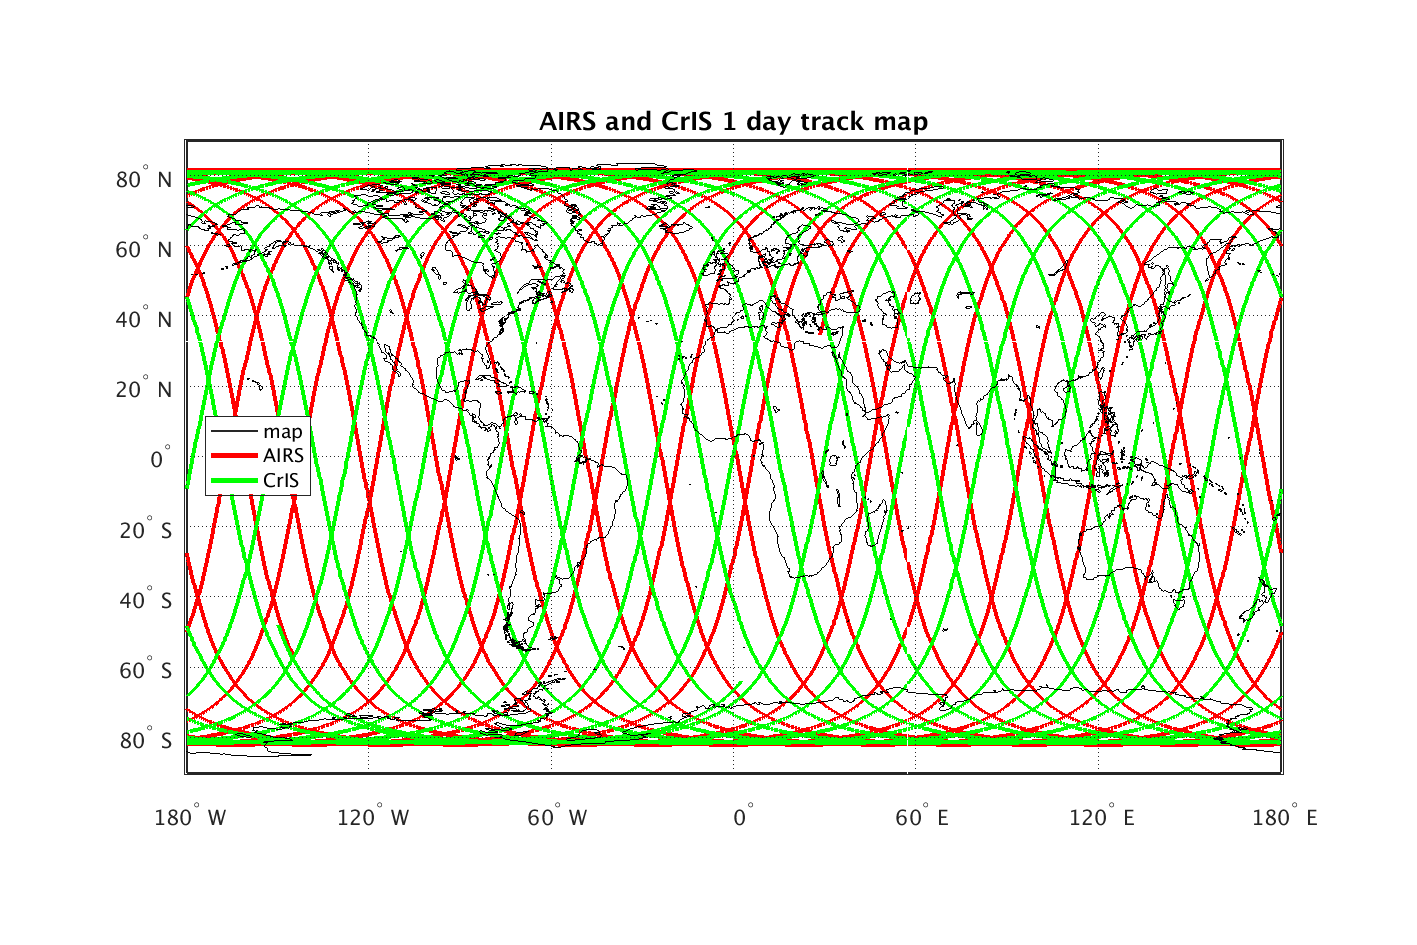
\includegraphics[width=\textwidth]{figures/subpt_1_day_all.png}
\vskip-12mm
\caption{Global one-day subpoint track map.}
\label{figD}
\end{figure}

% 16 day track maps
\begin{figure} % source plot_subpt.m
% \hskip-3.5cm
\centering
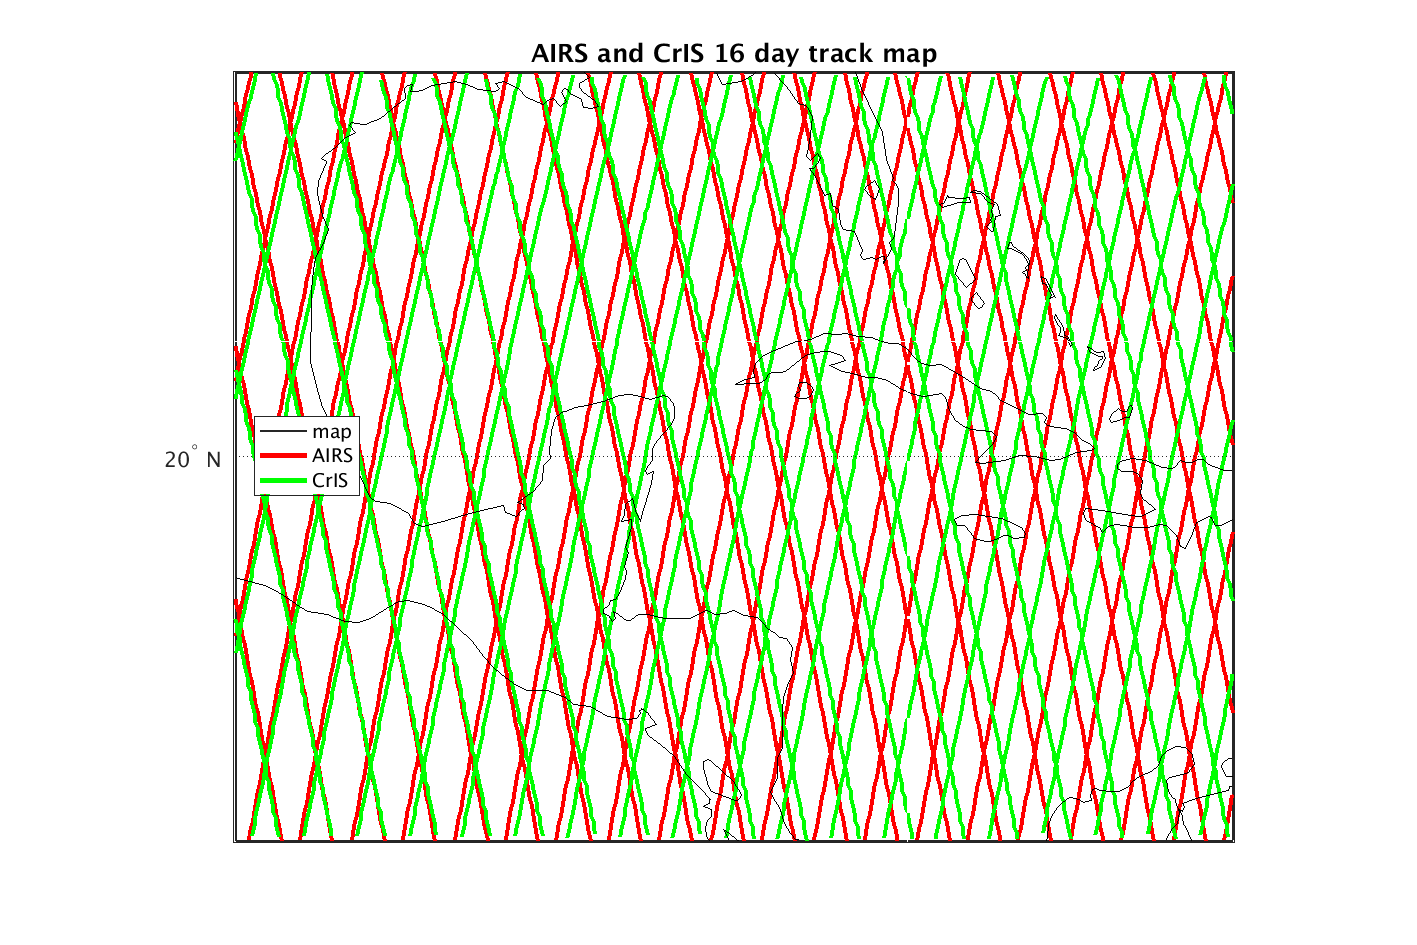
\includegraphics[width=\textwidth]{figures/subpt_16_day_zoom.png}
\vskip-9mm
\caption{Sixteen subpoint track map for the Caribbean.}
\label{figE}
\end{figure}

% AIRS and CrIS secant of zenith angles
\begin{figure} % source plot_tbin.m
\centering
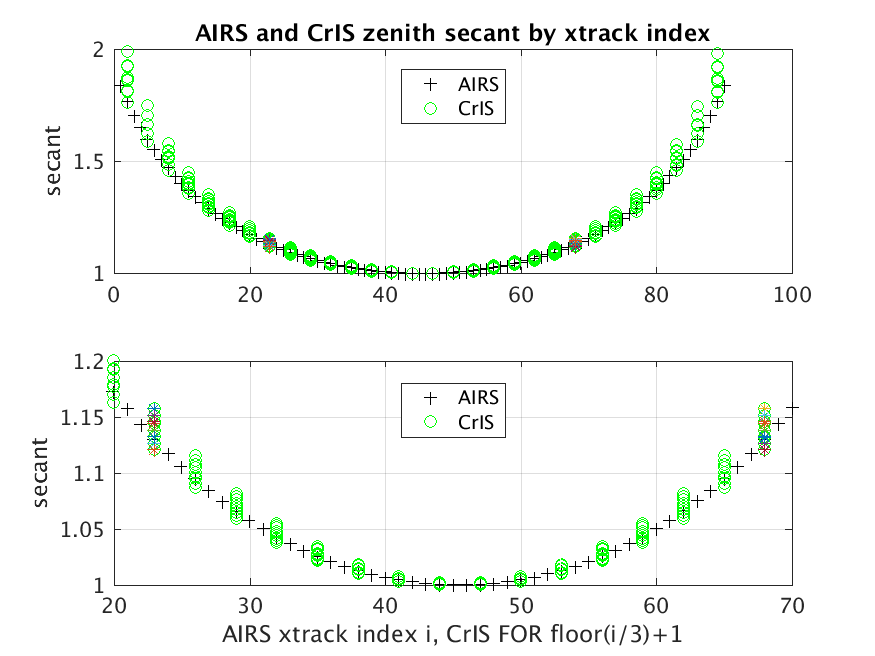
\includegraphics[width=\textwidth]{figures/AIRS_CrIS_secant_by_xtrack.png}
\caption{AIRS and CrIS secant of zenith angles}
\label{figF}
\end{figure}

AIRS L1c and CrIS L1b radiance data are organized as a sequence of
granule files, ordered by scan geometery and observation time.
Define an ``obs'' (observation) for AIRS as a single L1C 2645
channel radiance spectrum with an associated obs time, and for CrIS
as the the concatenation of the three radiance bands, giving $717 +
860 + 637 = 2214$ channels, again with a single associated obs time.
The AIRS L1c scan geometery is organized as 90 cross-track by 135
along-track observations, and so with 2645 radiance channels as an
$2645 \times 90 \times 135$ array.

The CrIS L1b scan geometery consists of 9 FOVs grouped in a $3
\times 3$ field of regard (FOR), giving 9 simultaneous observations,
with 30 cross-track FOR looks and 45 along-track steps.  With 2214
channels this can be represented as a $2214 \times 9 \times 30
\times 45$ array in the granule file.  (In practice this is broken
out by band, so we have a $717 \times 9 \times 30 \times 45$ array
for the LW, a $860 \times 9 \times 30 \times 45$ array for the MW,
and a $637 \times 9 \times 30 \times 45$ array for the SW.  But for
our basic counting here, we can simply use the concatenation.)

Note that $90 \times 135 = 9 \times 30 \times 45 = 12150$ gives us
obs per granule, for both AIRS and CrIS.  AIRS and CrIS spatial
sampling is similar, but not identical.  Both AIRS and CrIS are in
sun-synchronous polar orbits.  The CrIS orbital period is 101.5
minutes $\pm 0.2$ seconds, giving 227 orbits every 16 days.  The
AIRS orbital period 98.8 minutes, giving 233 orbits every 16 days.
Note that 227 and 233 are both prime; there are no common factors
and so no repeating subpatterns.

Figure \ref{figD} shows values for global satellite subpoint for
one day of AIRS and CrIS data, and figure \ref{figE} for 16 days,
the full period before any repeated postitions, for the Caribbean.
AIRS and CrIS are cross-track scanners, and in addition to subpoint
tracks we need to compare the scan geometry.  Figure \ref{figE}
shows the secant of zenith angles for AIRs and CrIS.  The upper plot
is for the full scan widths, while the lower is a near-nadir detail.
The general agreement is quite good, and the main difference we see
is due to the the CrIS FOV grouping.

Given our translations to a common 1679 channel radiance format,
the matching AIRS and CrIS obs count, with 12150 obs per granule,
and the generally similar sampling, we can define the CHIRP format
as an $1679 \times 12150$ array, channels by observation, in time
order.  Each ``obs'' has an associated values for time, FOV (for
CrIS), original indices for AIRS or CrIS, along with most of the
geo, support data, and product attributes from the parent sounders.
This involves some duplication of information for the individual
obs, but the overhead for this is small in comparison with the
radiance data.  CHIRP granules correspond with their parent AIRS or
CrIS granules, and inherit most of the parent granule's attributes
and supporting data.  CHIRP granules follow JPL conventions for
field names and attributes, and are saved in netCDF.

Aside from our basic CHIRP format, the representation as a list of
observations has some interesting applications.  For example we can
take a global tiling, and some time span, and associate each tile
with the obs that fall within it.  [CHIRP tiling is an obvious next
application.]

%----------- section --------------------------------------------------%
\section{CHIRP Quality Control and NEdN Estimates}

\subsection{AIRS-parent CHIRP QC}

\begin{itemize}

  \item We create two QC fields per granule, rad\_qc, a 12150-vector
    with one flag value per obs, and chan\_qc, a 1679-vector with one
    flag value per channel.  For both, 0 = OK, 1 = warn, and 2 = bad.
    rad\_qc is always 0 or 2, because AIRS L1c doesn't have a ``warn''
    flag.

  \item rad\_qc is set as a combination of the AIRS L1c field
    instrument\_state and sanity checks on radiance and geo values.

  \item chan\_qc is set to ``bad'' for those channels in the larger
    CHIRP 1679- channel set that are not part of the 1483 channel
    set translated from AIRS.

  \item chan\_qc is set to ``warn'' for the 6 channels at band edges.

\end{itemize}

\subsection{AIRS Synthetic Channels}

\begin{itemize}

  \item As an alternative to ``warn'' and to fill band gaps, AIRS
    L1c provides synthetic values for some channels.  These are
    flagged individually in the L1c file, and in addition there is a
    per-granule summary, L1cNumSynth, for each channel.

  \item We linearize the AIRS to CrIS translation and apply
    this to the AIRS values to get corresponding NumSynth values
    for CHIRP.  These are normalized as a fraction and becomes
    the CHIRP field synth\_frac.

  \item Then if $\hbox{synth\_frac} > 0.25$, we set chan\_qc to
    ``warn''.  The threshold $0.25$ is a parameter that can be changed
    in the production YAML specs.

  \item The following slides show the distribution of synthetic
    values from 20 days of AIRS data, and analogous values for
    synth\_frac from a representative CHIRP granule.

\end{itemize}

  \begin{centering}
  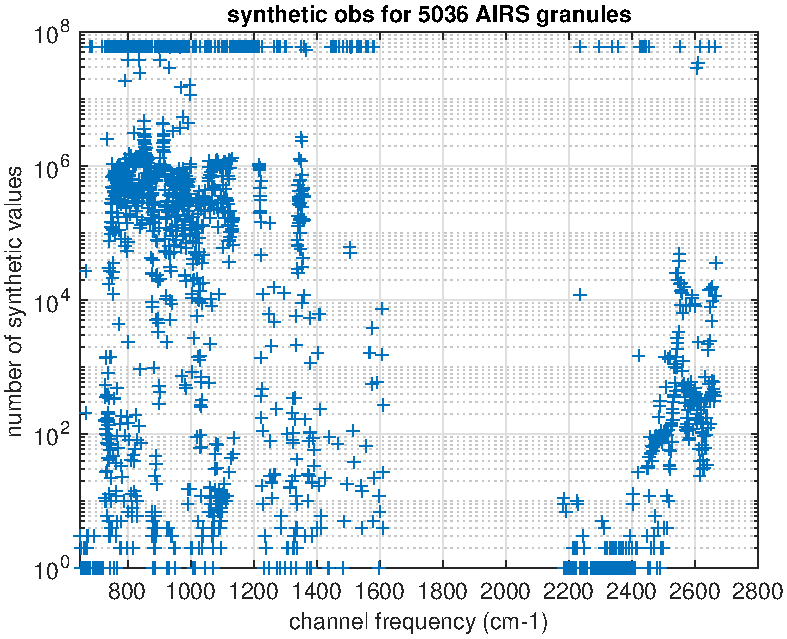
\includegraphics[width=\textwidth]{figures/synth_obs_freq_order.pdf}
  \end{centering}\vspace{3mm}

The sum of synthetic obs by channel for 5036 AIRS granules.
Counts are on a log scale.

  \begin{centering}
  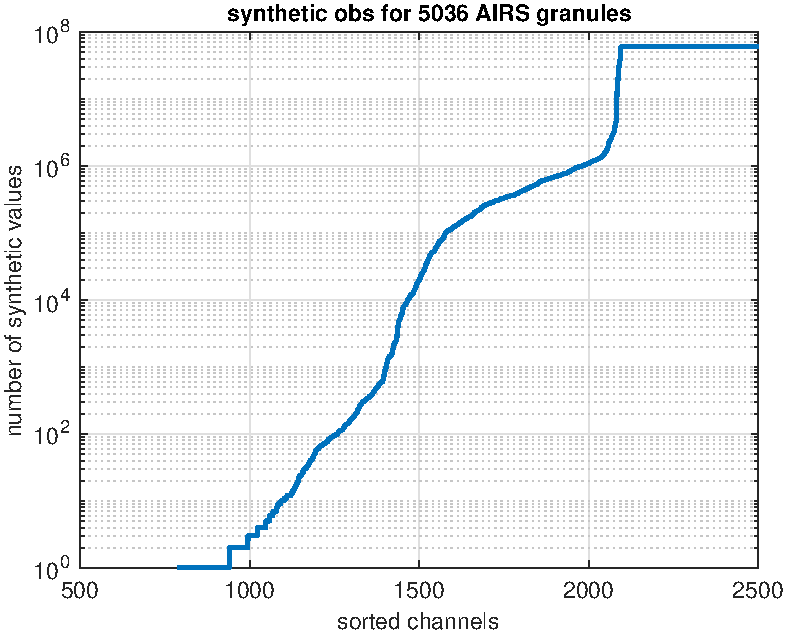
\includegraphics[width=\textwidth]{figures/synthetic_obs_counts.pdf}
  \end{centering}\vspace{3mm}

Synthetic obs per channel, sorted by number of synthetic obs.  This
shows the range of values.

CHIRP sample granule synth\_frac values

  \begin{centering}
  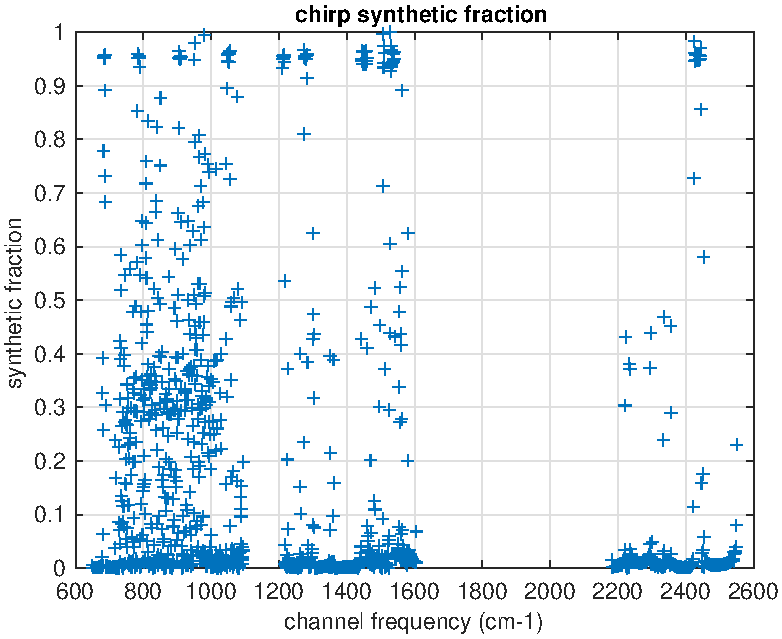
\includegraphics[width=\textwidth]{figures/chirp_sample_syn_frac.pdf}
  \end{centering}\vspace{3mm}

AIRS-parent CHIRP synthetic fraction for a single representative
granule.  This can be used to select channels with a relatively small
synthetic component.

  \begin{centering}
  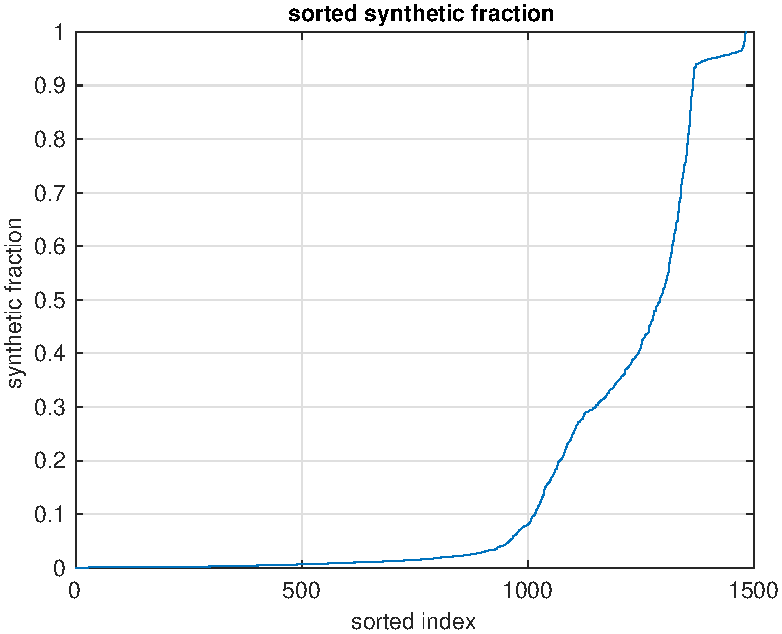
\includegraphics[width=\textwidth]{figures/chirp_sorted_syn_frac.pdf}
  \end{centering}\vspace{3mm}

AIRS-parent CHIRP synthetic fraction, sorted by synthetic
fraction magnitude.  This shows the variability of synth\_frac.

\subsection{AIRS-parent CHIRP NEdN}

\begin{itemize}

  \item {\nedn} for AIRS-parent CHIRP is estimated by adding
    simulated AIRS noise at 280K, doing the translation, and
    measuring the resulting noise.  This is done repeatedly and the
    mean of the measurement is reported.

  \item To get the AIRS estimate, we take the mean of valid
    {\nedn} values over an AIRS granule, and interpolate over
    gaps from the synthetic channels.  AIRS L1c does not provide
    an {\nedn} estimate for these channels, so perhaps this is the
    best we can do.

  \item More detail on the noise estimate is provided in the IEEE TGRS
    AIRS deconvolution paper, mentioned above.

  \item The correlated fraction of AIRS noise varies from module
    to module, and is significant for some modules.  The translation
    will preserve this correlation.  {\nedn} estimates for such
    cases are a matter for future work.

\end{itemize}

\subsection{AIRS and CrIS parent CHIRP NEdN}

  \begin{centering}
  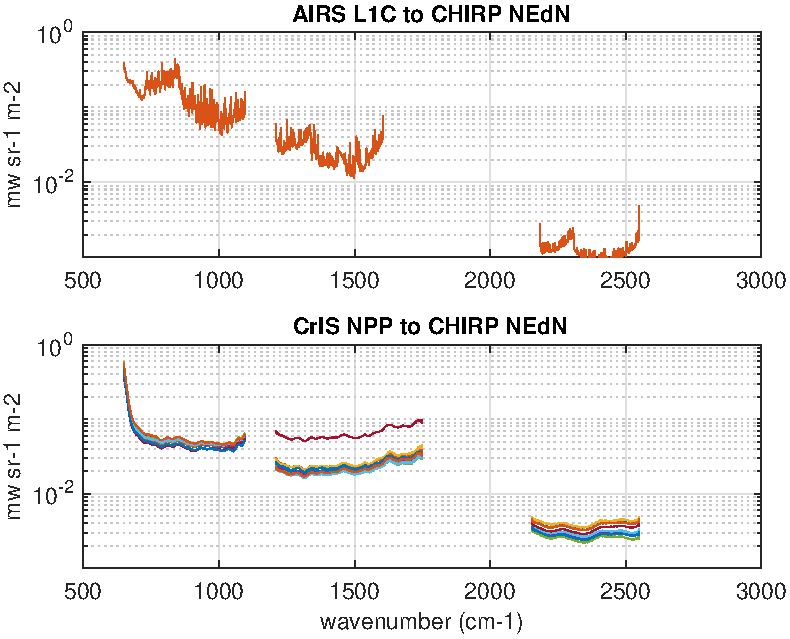
\includegraphics[width=\textwidth]{figures/chirp_nedn_from_airs_and_cris.pdf}
  \end{centering}\vspace{3mm}

Sample CHIRP {\nedn} for AIRS and CrIS parent data, 2018 doy
231 granules 25 and 21, two relatively warm granules.

  \begin{centering}
  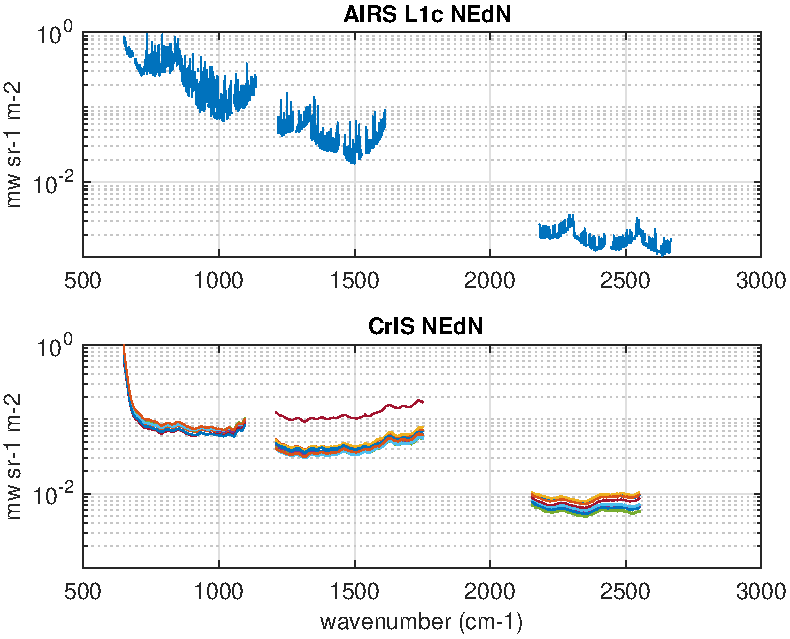
\includegraphics[width=\textwidth]{figures/sample_airs_and_cris_nedn.pdf}
  \end{centering}\vspace{3mm}

Sample AIRS and CrIS {\nedn} for the same two granules, 2018 doy
231 granules 25 and 21.

\subsection{CrIS-parent CHIRP NEdN and QC}

\begin{itemize}

  \item In comparison with AIRS, estimating CrIS-parent
    CHIRP {\nedn} and doing QC is relatively simple.

  \item CrIS-parent CHIRP {\nedn} is derived from the high
    res CrIS {\nedn} with scale factors to take into account the
    interpolation and apodization.  These are
    \begin{itemize}
      \item LW, 0.6325, for Hamming apodization only
      \item MW, 0.5455, for interpolation and Hamming apodization
      \item SW, 0.4446, for interpolation and Hamming apodization
    \end{itemize}

  \item CrIS-parent CHIRP QC is determined from the CrIS
    parent, by combining the fields for the individual CrIS bands.

  \item chan\_qc is set to 0 (OK) for CrIS-parent CHIRP.

  \item possibly we should set chan\_qc to ``warn'' at the band
    edges, as we do for AIRS parent, but we are not doing this
    now.

\end{itemize}

%----------- section --------------------------------------------------%

\section{Conclusions and Future Work}
\begin{itemize}

  \item This talk can serve as a draft for a significant part of the
    CHIRP User's guide.

  \item Future work includes refining bias vectors and taking
    account of AIRS correlations in the {\nedn} estimates.

  \item Closely related work includes future gridded products, which
    share many parts with the CHIRP L1c processing.


\end{itemize}

%----------- section --------------------------------------------------%

\end{document}

